\documentclass{/home/janmebows/Documents/LatexTemplates/myassignment}


%%Document info
\title{Disease Dynamics (App Topic B)}
\begin{document}

\setlength{\parindent}{0pt}
\maketitle

\section{Introduction}
This course is about epidemiology - epidemics being a widespread activity/outbreak within a region/community. We will be considering epidemics of infectious diseases and just refer to them as epidemics.\\

At a community (population/household/school) level:\\
The data we get is symptom onset data - if they get infected at time $0$, there will be some time where the first persons infection/symptoms are visible (primary symptomatic case/index case). After some period of time you could have the the secondary symptomatic case (next person shows symptoms).
The time interval between the first and second symptomatic cases is referred to as the serial interval. \\

Individual level:\\
We look at their viral load - how much of the virus/bacteria/etc. is within the person.
At some point they get infected and the viral load increases logistically and then decreases exponentially. There could be a residual load of viral load, viral load could get large enough to kill the individual, other cases can occur. We consider a threshold where you have to be above that threshold to become infectious. There would be another threshold where symptoms are displayed (does not necessarily have to be after becoming infectious).
When the viral load drops below the threshold, the infectiousness ends.\\

The period before being infected is the \textbf{susceptible} period.\\
After being infected, and preceding the infectious threshold is the \textbf{latent/exposed} period.\\
The time between being infected and showing symptoms is the \textbf{incubation} period.\\
The time while infectious until the dropping below the viral load threshold is the \textbf{infectious} period.\\ 
Following the infectious period you are considered to be in the \textbf{recovered} period. For some diseases this puts you back into the \textbf{susceptible} period.\\

We want to map this information to a mathematical model, and we do this by mapping the \textbf{periods} to \textbf{compartments} or groups.\\


Compartmental models:


Each individual belongs to one (and only one) of the compartments:
\begin{itemize}
    \item S - susceptible
    \item E - exposed
    \item I - infectious
    \item R - recovered
\end{itemize}
Notation for models:
\[S\to I \to R\]
\[S\to I\to S\]
\[S\to E\to I\to R\]
For some examples.


Other features/characteristics of models:
\begin{itemize}
    \item State - \textbf{discrete} or continuous-approximation (large population)
    \item Time  - discrete or \textbf{continuous}
    \item Variability/Stochasticity - \textbf{present} or absent (stochastic / deterministic)
\end{itemize}

We will mostly consider discrete state with continuous time where variability is present.


\section{Deterministic Models I}
Consider a population with a fixed number of individuals, $N$. Let the population of individuals be identical, And a disease with an $S-I$ dynamic.\\
Let $I$ be the number of infectious individuals, $S$ the susceptible and $F$ be the force of infection (per-capita rate at which susceptibles become infected).
$F$ should depend on time, the number of people infected, how people interact, and how infectious the disease is. Note that $S = N-I$, due to this, for the state we only care about $I$
\begin{table}[h]
    \centering
    \begin{tabular}{c|c|c}
         Event&$\Delta$State&Rate  \\
         \hline
         Infection&$I\to I+1$&$FS= F(N-I)$
    \end{tabular}
    \caption{Example model}
\end{table}

According to Begon et al. (2002), $F = c\times p \times q$ where 
\begin{itemize}
    \item c - rate at which an individual makes contact with other individuals with potential for transmission. 
    \item p - the probability that a contact is with an infectious individual. In this case since they are all identical: $\frac{I}{N}$ (homogeneous-mixing model/law of mass action)
    \item q - the probability that the infection is transmitted to the other individual
\end{itemize}
There are 2 commonly used forms for $c$: density dependent transmission (DDT) and frequency dependent transmission (FDT).\\
DDT: the rate of contacts increases with population density: $K$ is a constant, and $A$ is the area
\[c = K\frac{N}{A}\]

FDT: the rate of contacts is a constant $\beta$.

If we hold $N$ constant, then DDT becomes an FDT, and for some scenarios it makes more sense to use one over the other.

For F we consider:

\[F= \begin{cases}
\beta \frac{I}{N}&FDT. \quad (\beta = K\times q)\\
\beta I& DDT.\quad (\beta = \frac{K\times q}{A})
\end{cases}\]
Writing deterministically:\
\[\textit{Rate of change of state }= \sum_{Events}\Delta\textit{State }\times \textit{ Rate }\] 
\[\frac{dI}{dt} = \begin{cases}
\beta \frac{I}{N}(N-I),&FDT.\\
\beta I(N-I),&DDT.
\end{cases}\]

Should work with proportions (assuming $N$ is suff large).
Let $i := \frac IN$
Giving
\[\frac{di}{dt} = \begin{cases}
\beta i(1-i),&FDT.\\
\beta Ni(1-i),&DDT.
\end{cases}\]
\newpage
Now if we consider the SIS model with a fixed population size, and assume frequency dependent transmission:
\begin{table}[h]
    \centering
    \begin{tabular}{c|c|c}
         Event&$\Delta$ State&Rate \\
         \hline
         Infection&$I=I+1$&$\beta I\frac{(N-I)}{N}$\\
         Recovery &$I=I-1$&$\gamma I$
    \end{tabular}
\end{table}

Where $\gamma$ is the per-individual rate of recovery. Meaning
$\frac1\gamma$ is the average infectious period for an individual.
This gives the ODE (in terms of proportion):
\[\frac{di}{dt} = \beta i(1-i) - \gamma i\]

Now the SIR model with FDT:\\
Now we care about both S and I ($N$ is still fixed). Where $R = N - (S+I)$.
If we let the statespace be $(S,I)$:
\begin{table}[h]
    \centering
    \begin{tabular}{c|c|c}
         Event&$\Delta$ State&Rate \\
         \hline
         Infection&$(S-1,I+1)$&$\beta I\frac{S}{N}$\\
         Recovery &$(S,I-1)$&$\gamma I$
    \end{tabular}
\end{table}

Since this is now bivariate we have a coupled system of ODEs:
\begin{align*}
    \frac{dS}{dt}&=-\beta I\frac{S}{N}\\
    \frac{dI}{dt}&= \beta I \frac{S}{N} - \gamma I
\end{align*}
Or in terms of proportions ($s:=\frac{S}{N}$)
\begin{align*}
    \frac{ds}{dt}&=-\beta is\\
    \frac{di}{dt}&=\beta is - \gamma i
\end{align*}

For the SI model what do we expect to happen?
$i$ is monotonically increasing, and we expect that as $t\to\infty$, $i\to 1$.
O\\
By analytically solving the DE we get:
\[i(t) = \frac{i_0}{i_0 + (1-i_0)e^{-\beta t}}\]
Where $i(0) =i_0$. Which makes this limit clear.

Since $i \sim $ as $t\to \infty$ how do we describe when the outbreak is complete?\\
One way is (let $T_1$ be the time the outbreak ends:
\[T_1 = \inf\{t | i(t) > 1-\frac{1}{N}\}\]
I.e. it is complete when there is less than 1 person left.
\begin{align*}
    i(T_1) = \frac{i_0}{i_0+(1-i_0)e^{-\beta T_1}} & > 1-1/N\\
    i_0 &= (i_0+(1-i_0)e^{-\beta T_1})(1-1/N)\\
    i_0&=i_0 - i_0/N + (1-i_0)e^{-\beta t}\\
    \vdots\\
    T_1&= \frac{1}{\beta} \log\left(\frac{(N-1)(1-i_0)}{i_0}\right)
\end{align*}
Think about what happens when the parameters are changed.
We would expect if we increase $\beta$ the outbreak would complete faster, so $T_1$ should be smaller (which works). If we increase $N$, it would take longer to complete so $T_1$ would be larger (good).


Now if we look at the SIS model:


The long-term dynamics of this model depend on the `basic reproduction number', $R_0$, the (expected) number of secondary infections caused by one infected individual in an otherwise entirely susceptible population. $R_0$ is a threshold parameter. You would expect if $R_0 < 1$ then the outbreak will die out. If $R_0 >1$ then it is possible to blow up. For this model:
\[R_0 = \frac\beta\gamma   \quad \textit{(linearisation for large } N \textit{)} \]


Theorem:
Let $i(t)$ be a solution to the SIS model
\begin{enumerate}
    \item If $R_0 \leq 1$, then $\lim_{t\to\infty} i(t) = 0$ (disease free equilibrium)
    \item If $R_0 > 1$, then $\lim_{t\to\infty} i(t) = 1 - \frac{1}{R_0}$ (endemic equilibrium)
\end{enumerate}


Now the SIR model with FDT:\\
\begin{align*}
    &\frac{ds}{dt} = -\beta si\\
    &\frac{di}{dt} = \beta si - \gamma i
\end{align*}
Recall $\beta$ is the effective transmission rate parameter and $\frac1\gamma$ is the average infectious period.\\
From a paper we get:\\
\textbf{Threshold result: }
\begin{align*}
    \frac{di}{dt} &= \beta si - \gamma i\\
    &= \beta i(s - \frac\gamma\beta)\\
    &= \beta i(s - \frac1R_0)
\end{align*}
Hence if $s(0) < \frac1R_0$, $\frac{di}{dt} < 0$. I.e. the infection will monotonically die out, if the initial proportion of susceptibles is less than $\frac1R_0$.
How could we exploit this for public health? Decrease the effective number of susceptibles (HERD IMMUNITY). So you would want at least $(1-\frac{1}{R_0}) < 100\%$ of the population vaccinated.

\textbf{Escape result:}
Why does the epidemic end? While not necessarily required for describing the dynamics of the epidemic
\[\frac{dr}{dt} = \gamma i\]
Where $r$ is the proportion of the recovered individuals.

\[\frac1s \frac{ds}{dt} = -\frac\beta\gamma \frac{dr}{dt} = -R_0 \frac{dr}{dt}\] 
By considering the left and right (not the middle), integrating, exponentiating and applying the initial condition $(s(0) = s_0, i(0) = i_0, r(0) = 0$, we get:
\[s = s_0 e^{-r(t)  R_0}\]



\begin{align*}
    \frac{di}{dt} &= \beta si - \gamma i\\
    &\geq  -\gamma i\\
    \implies i(t) &\geq i_0 e^{-\gamma t}
\end{align*}

This is always positive, and the limit $t\to \infty$ will tend to $0$.
So since $i \geq 0$, and $\frac{dr}{dt} = \gamma i$ then $\frac{dr}{dt > 0}$ for all $t<\infty$.
And since $s(t)$ relies on $r(t)$ it is strictly decreasing, and is bounded below by $0$.\\
Hence, $s(t)$ converges to a finite limit, $s_\infty$. Since $s$ converges, $r$ must also converge. 
Since $i$ must converge, $\frac{dr}{dt}$ must approach $0$, and thus $i_\infty = 0$.

The number of infectious individuals will decline and that causes the end of the epidemic. This does not happen due to an absence of susceptibles.

\[s_\infty = s_0 e^{-r_\infty R_0}\]

\textbf{Final Size:}
We know that 
\[r_\infty = 1-s_\infty = 1-s_0 e^{-r_\infty R_0}\]
\[\implies r_\infty = 1 + \frac1{R_0} W (-s_0 R_0 e^{-R_0})\]
Where $W(\cdot)$ is the principal branch of the Lambert-W function (omega function apparently)
The Lambert-W function is the inverse of
\[f(x) = xe^{x}\]

An approximate solution:
\begin{align*}
    \frac{ds}{dt}&= -\beta si\\
    \frac{di}{dt}&= \beta si - \gamma i\\
    \frac{dr}{dt}&= \gamma i
\end{align*}
Use the 3rd equation and a Taylor expansion (truncate after the squared term):
\[e^{-u} = 1 - u + \frac{u^2}{2} + \hdots\]
\begin{align*}
    \frac{dr}{dt}&=\gamma i\\
    &= \gamma(1-r-s)\\
    &= \gamma(1-r-s_0e^{-rR_0})\\
    &\approx \gamma\left(1-r-s_0\left(1-rR_0 + \frac12 r^2 R_0^2\right)\right)\\
    &\approx \gamma(1-s_0 + r(s_0R_0 - 1) - \frac{r^2R_0^2s_0}{2})\\
    &\approx \frac{\gamma}{2s_0R_0^2} \left((1-s_0)2s_0R_0^2 + (s_0R_0-1)^2 - \left[s_0R_0(r-\frac{1}{s_0R_0^2}(s_0R_0-1))\right]^2\right)\\
    &\approx \frac{\gamma}{2s_0R_0^2}\left(\alpha^2 - \left[s_0R_0(r- \frac{1}{s_0R_0}(s_0R_0-1))\right]^2\right)
\end{align*}
Where $\alpha = \left(2s_0R_0^2 (1-s_0) + (s_0R_0-1)^2\right)^{1/2}$\\
The next step which makes no sense uses:
\[\alpha \tanh(v) = s_0 R_0^2 [r- \frac{1}{s_0R_0^2}(s_0R_0-1)], \quad r(0)=0 \implies \alpha \tanh(v(0)) = -(sR_0-1) \]
Rearranging gives
\[r = \frac{\alpha}{s_0R_0^2} \tanh v + \frac{1}{s_0R_0^2}(s_0R_0-1) \]
We also differentiate it:
Note we are not expected to reproduce this result

\begin{align*}
    \frac{dr}{dt}&\approx \frac{\gamma}{2s_0R_0^2} \left[\alpha^2 - \alpha^2 \tanh^2v\right]\\
    &\approx \frac{\alpha}{s_0R_0^2} \text{sech}^2v \frac{dv}{dt}\\
    \implies \frac{dv}{dt} &= \frac{\gamma \alpha}{2}\\
    \implies v(t) &= \frac{\gamma\alpha t}{2} + v(0)\\
    \implies r(t) \approx \frac{1}{s_0R_0^2} (s_0R_0-1) + \frac{\alpha}{s_0R_0^2} \tanh \left(\frac{\gamma\alpha t}{2} - \phi\right)
\end{align*}
Where $\phi = \tanh^{-1}(\frac1\alpha (s_0R_0-1))$

Fuck that.

When do we expect this approximation to be accurate?
The only approximation was by truncating the taylor series, which means it'll be small if $u$ is small. In this case $u = rR_0 < 1$ (he said 1 wasn't great though). So we want $r < \frac{1}{R_0}$
So we want small $R_0$. 


\textbf{Early Dynamics:}
If the population is very large, in the early stages most people will be susceptible. I.e. $s\approx 1$
\[\implies \frac{di}{dt} \approx \beta i -\gamma i \approx (\beta-\gamma)i\]
\[\implies i(t) \approx i_0 e^{(\beta-\gamma)t}\]
So the early growth rate is $r = \beta-\gamma$


\section{CTMCs}
Objectively the worst thing we could be doing right now.
Theory revision:

CTMC defined as a discrete-state, continuous time, stochastic process which satisfies the markov property.\\
Markov Property:
\[P(\textit{future}\Bigm| \textit{present, past}) = P(\textit{future}\Bigm| \textit{present}) \]

Let $X(t) = (X(t),t\geq 0)$ be a continuous time stochastic process. Let $X(t) \in S$ $\forall t \geq 0$, where $S$ is the state space and we will assume $S$ is countable. We will also work with only finite $S$ in this course which is nice.

$X(t)$ is called a markov chain if for all finite sequences of times: $0<t_1<\hdots<t_n<t_{n+1}$ and states $j_1,\hdots,j_{n+1} \in S$, we have
\[P(X(t_{n+1}) = j_{n+1} | X(t_n) = j_n, \hdots X(t_1) = j_1) = P(X(t_{n+1}) = j_{n+1} \Bigm| X(t_n) = j_n)\]
We can answer any question we'd like about $X(t)$ if we knew its transition function
\[P_{ij}(s,t+s) = P(X(t+s)=j \Bigm| X(s) = i)\]
\[P(s,t+s) = (P_{ij}(s,t+s), \forall i,j\in S,s,t \geq 0 )\]

Obviously this is a tad hopeful.

The chain is time homogeneous if the transition function only depends on time through the time step. I.e. if the above does not depend on $s$.
\[P_{ij}(s,t+s) = P_{ij}(0,t) =: P_{ij}(t)\]
We will only consider time homogeneous problems.

A set $P= p_{ij}(t)$ of real valued functions is called a transition function if
\begin{enumerate}
    \item $P_{ij}(t) \geq 0$ for all $t\geq 0$
    \item $P_{ij}(0) = \delta_{ij}$ $\delta_{ij} =1$ if $i=j$, $0$ if $i\neq j$.
    \item $\sum_{j\in S} P_{ij}(t) \leq 1$ for all $t\geq 0$
    \item $P_{ij}(t+s) = \sum_{k\in S} P_{ik}(s) P_{kj}(t)$
\end{enumerate}
The 4th is the Chapman-Kolmogorov equations (uses LOTP and time homogeneity)
Note that for the $3rd$ we used $\hdots \leq 1$, there are some interesting properties with countable sets which put in the less than part. 


More CTMC garbage:

Recall for the ODE models we didn't specify $i(t)$ directly. We specified the instantaneous rate of change of $i$


For CTMCs, we want to know the transition function which we can't typically specify it. However we are likely to be able to specify (and estimate) the instantaneous transition rates.

For the SI model as a CTMC it is much the same as the ODE, I.e. the state space is $I(t)$ (number of infectious). Where $I(t) \in [0,N] \subset Z$ where $N$ is the population size.
The only event is $I\to I+1$ at rate $\beta I(N-I)/(N-1)$


We typically use $q_{ij}$ to represent the transition rates from $i$ to $j$. So in this case
\[q_{ij} = \begin{cases}
\beta I(N-I)/(N-1), & j=i+1\\
-\beta I(N-I)/(N-1), & j=i\\
0, & otherwise
\end{cases}\]


We define the matrix $Q = (q_{ij}, i,j \in S)$ as the q-matrix / transition-rate matrix / generator. 

We find the rates relate to $P$. \\
As a theorem: Let $P$ be a standard transition function, meaning
\[\lim_{t\to 0^+} P_{ij} = \delta_{ij}\]
Then we have:
\[q_{i} : = \lim_{t \to 0^+} \frac{1-P_{ii}(t)}t\ exists \ \forall i,\ 0\leq q_i \leq \infty\]
\[q_{ij} := \lim_{t\to 0^+} \frac{P_{ij}}t\ exists\ \forall j\neq i,\ 0\leq q_{ij} < \infty\]
Where $q_{i} = \sum_{\substack{j\in S\\j\neq i}} q_{ij}$
Then the limit exists and $0\leq q_i \leq \infty$ (we will assume this is less than $\infty$ for this course).
We aren't proving this ourselves.

Time for the KFDEs/KBDEs... Using the Chapman Kolmogorov equations we get the forward equation:
\begin{align*}
P_{ij}(t+s) &= \sum_{k\in S} P_{ik}(s) P_{kj}(t)\\
P_{ij}(t+s)&= \sum_{k\neq j} P_{ik}(s) P_{kj}(t) + P_{ij}(s) P_{jj}(t)\\
\implies P'(t) &= P(t)Q
\end{align*}
We get this last step by subtracting $P_{ij}(s)$, dividing by $t$ and then considering the limit as $t\to 0$. We can swap the order of the limit and the sum since we're assuming finite.


If $Q$ is regular (non-explosive) (finite state space is a sufficient condition). We can get the backward equation

Forward:
\[P'(t) = P(t)Q\]
Backward:
\[\]


Don't forget our solutions given the forward equation is
\[P(t) = P(0) e^{Qt}\]
Where $e$ is the matrix exponential:
\[e^{Qt}: = \sum_{n=0} Q^n \frac{t^n}{n!}\]
Note $P_{ij}(0) = \delta_{ij}$ So $P(0) = I$
So out solution is
\[P(t) = e^{Qt}\]

Given an initial probability mass function over $S$, $P(0) = (p_i(0),\forall i\in S)$ Then we get:
\[p(t) = p(0)e^{Qt}\]
Where $p(t)$ is the probability of being in any particular state at time $t$.

Using this method would work computationally but would not be overly efficient.

If we differentiate with respect to time 
\[\frac{dp(t)}{dt} = p(t) Q\]
Which would be solved with an ode solver... \verb|ode45|. This is the forward equation or master equation


Classifying states: consider states $i,j \in S$ 


Communicating class if there exists a finite sequence $k_1,\hdots,k_n$ distinct from each other, s.t.
\[q_{ik_1} \times q_{k_1k_2} \times \hdots \times q_{k_n j} > 0\]
Then $i$ leads to $j$ ($j$ is accessible from $i$) We will denote this with $i\to j$.
If we also have the other way around, $j\to i$. Then they are communicating states, denoted
\[i\leftrightarrow j\]
Communication is an equivalence relation. Transitive, symmetric, reflexive:

$i\leftrightarrow j$ iff
\begin{enumerate}
    \item $i \leftrightarrow j$ $\Leftrightarrow$ $j\leftrightarrow i$ (symmetric)
    \item $i\leftrightarrow i$ (reflexive)
    \item $i\leftrightarrow j$ and $j\leftrightarrow h$ $\implies$ $i\leftrightarrow h$ (transitive)
\end{enumerate}
This means that communication partitions the state space $S$ into a set of communicating classes.

Some random definitions:
\begin{itemize}
    \item A class $B \subseteq S$ is irreducible if $B$ is a communicating class. If $B = S$ then the CTMC is said to be irreducible.
    \item A class $C$ is closed (absorbing) if for any state $i\in C$ and $i \to j$ then $j \in C$. I.e. you can't leave $C$ once entered.
    \item A state $i$ is an absorbing state if $i$ is a closed class. I.e. $q_{ij} = 0 \ \forall j$
\end{itemize}

A state $j$ is transient if
\[\int_0^\infty P_{jj}(t) dt < \infty\]


A state $j$ is recurrent if
\[\int_0^\infty P_{jj}(t) dt = \infty\]
$j$ is positive recurrent if: (letting $T_{jj}$ be the return time)
\[E[T_{jj}] < \infty \]

$j$ is null recurrent if:
\[E[T_{jj}] = \infty\]


\section{CTMC Epidemic Models}
The SI model as a CTMC:
$I(t)$ - number of infectious individuals. Where the only event is infection $I\to I+1$ occurring at the rate $\beta I(N-I)/(N-1)$. The $N-1$ is necessary for small $N$, to exclude the one person in contacts (in a population of one, the rate is 0...)

State space $S = \{I : 0\leq I \leq N\}$ Where $I(0) = I_0 = 1$

Forward equation for this process:
\[\frac{dP_I(t)}{dt} = \begin{cases}
0,& I=0\\
P_{I-1}(t)q_{I-1,I} - P_{I}(t) q_{I}& 1\leq I \leq N-1\\
P_{N-1}(t) q_{N-1,N}& I=N
\end{cases}\]
Note this process is a series of individual transient states (no communicating classes). $0$ and $N$ are absorbing classes.

Alternatively using the $Q$ matrix:
We will have the first row is zeros, and then the diagonal (and upper diagonal) are non-zero, with all other parts are zeros.
Recall the row sums are zero.

Now for the SIS model:\\
Same $I$ same $S$ as last time. The events are infection ($I\to I+1$ at the same rate as before) and recovery ($I\to I-1$ at rate $\gamma I$). $0$ will still be an absorbing state, and all the other states form an irriducible transient communicating class.
Forward equation for this process:
\[\frac{dP_I(t)}{dt} = \begin{cases}
P_{1} q_{1,0},& I=0\\
P_{I-1}(t)q_{I-1,I} - P_{I}(t) q_{I}& 1\leq I \leq N-1\\
P_{N-1}(t) q_{N-1,N}& I=N
\end{cases}\]

The $Q$ matrix will be the same but there will also be a lower diagonal (it is a tridiagonal matrix).

For large $N$, $Q$ is a sparse matrix. In matlab $Q = sparse(N,N)$ and then fill in the matrix 



For the SIR model:\\
($S(t),I(t)$) - bivariate CTMC.
\[S = \{(S,I) \in \mathbb{Z}^2 : 0 \leq S,I,S+I\leq N\}\]
Possible events:\\
Infection $(S-1,I+1)$ at rate $\beta IS/(N-1)$\\
Recovery $(S,I-1)$ at rate $\gamma I$

For this process there will be $N+1 +N + N-1 + \hdots + 1$ states. With $N+1$ zero states in this case.
So for a $1-1$ mapping to the integers we would take $(S,I)$ maps to the $1 +S + NI^{th}$ row.


\subsection{Degree-of-advancement representation (Event count / reaction count representation)}
So far we have specified models using the \textbf{population representation}. E.g. $I(t)$ for SIS, $(S,I)$ for the SIR model. These consider the numbers of individuals in the population - this is the natural way to think about it - but there's an alternative representation.

DA representation keeps track of the number of events of each type that have occurred. I.e. the process will be an n-variate process where $n$ is the number of event types.

E.g. SIS model: $z_1(t)$ is the number of infection events and $z_2(t)$ is the number of recovery events. To recover the initial information that we want i.e. the population after $t$ then we can map to the population
\[I(t) = I(0) + z_1 - z_2\]
This does make us use a bivariate process (instead of univariate), but we do keep track of more information this way.

For the $SIR$ model we have the same $z_1$ and $z_2$ - so it is bivariate, but now we have extra information without increasing the number of variables
\[I(t) = I(0) + z_1 - z_2\]
\[S(t) = S(0) - z_1\]

The state space is for the SIR model (this might be wrong)
\[S = \{(z_1,z_2) \in Z^2 | 0 \leq z_2 \leq z_1 + I(0), 0 \leq z_1 \leq S(0)\}?\]
To clean this up we usually incorporate $I(0)$ and $S(0)$ into $z_1,z_2$ to save a lot of hassle.
So from now on $z_1,z_2$ will include them.

When $z_1 = z_2$ it corresponds to an absorbing state.


Soon we will look at obtaining $Q$.

\[\frac{dp}{dt} = pQ\]
Which is a system of linear ODEs, giving
\[p = p(0) e^{Qt} \]

Numerical approaches to solve this: We could either use the system of DEs, or use the matrix exponential and approximate it.

If we use the system of linear ODEs, we could use for example \verb|ode45()| (which is a Runge-Kutta method)

An alternative is the implicit-Euler (IE) method. 
the IE method is effective if $p(s)$ is not changing too much. We would expect the approximation to improve as $\tau \to 0$.

\[p(s+\tau) - p(s) = \int_s^{\tau +s} p(t) Q dt \approx \tau p(s+\tau) Q\]
\begin{align*}
    \hat{p}(s+\tau)[I - \tau Q] = \hat{p}(s)\\
\end{align*}
So we would solve this in matlab as
\[\hat{p}(s+\tau) = \hat{p}(s)/[I - \tau Q] \]
And we would want to keep $\tau$ small and iterate this.
If we wanted to run it over a period $t$, recursively solve this $t/\tau$ times.
What value of $\tau$ is acceptable? Consider $p(s+\tau) = p(s) e^{Q\tau}$
So we want
\[e^{-Q\tau} = I-\tau Q + \mathcal{O}(\tau^2)\]
So the local truncation error is $\mathcal{O}(\tau^2)$, and the global error at $t$ (we won't derive this) is $\mathcal{O}(\tau)$


This method produces a probability vector for all $\tau$. 
There is another nice feature which we will mention on thursday


Matrix Exponential:
For small matrices, the `best' method is `scaling and squaring', with `Pad\'e approximant' to $e^x$. This is effectively what Matlab uses in \verb|expm()|. For larger (and sparse) matrices, the `best' method is the `Krylov subspace method'. 

There is a software package for computing the matrix exponential `EXPOKIT' which uses the krylov subspace to do this.
\[p(t) = e^{tQ}p_0 = p_0 + (tQ)p_0 + \frac{(tQ)^2}{2} p_0 +\hdots\]
And approximate this using an element of the krylov subspace
\[\mathcal{K}_m(A,v) = span\{v,Av,\hdots,A^{m-1}v\}\]
Where $m$ is the dimension (order of the subspace) and it is small compared to the order of the matrix $A$.



Considerations for implementation:
Often we want to investigate a model with the same population size $N$, but with different parameters ($\beta,\gamma,\hdots$). This is certainly the case for inference. Note that the rates are linear in the parameters with one parameter for each event.
Hence it will be more efficient to use
\[Q = \beta Q_1 + \gamma Q_2\]
Where $Q_1$ is the generator for the chain with just infection events, and $Q_2$ is that for recovery events. So this way, $Q_1$ and $Q_2$ can be formed once and stored.

\clearpage
Sensible ordering of states for multidimensional problems is lexicographical (or co-lexicographical) ordering. In the latter,
\[(a,b) \prec (a',b')\]
\[iff \ b < b' \ or \  b = b' \ \& \ a < a'\]


So for the SI model it becomes
\begin{table}[h]
    \centering
    \begin{tabular}{c|c}
         $j$&$(S,I)$ \\\hline
         1&(0,0)\\
         2&(1,0)\\
         3&(2,0)\\
         4&(3,0)\\
         5&(0,1)\\
         6&(1,1)\\
         7&(2,1)\\
         8&(0,2)\\
         9&(1,2)\\
         10&(0,3)\\
    \end{tabular}
        \begin{tabular}{c|c}
         $j$&$(S,I)$ \\\hline
         1&(0,0)\\
         2&(1,0)\\
         3&(2,0)\\
         4&(3,0)\\
         5&(1,1)\\
         6&(2,1)\\
         7&(3,1)\\
         8&(2,2)\\
         9&(3,2)\\
         10&(3,3)\\
    \end{tabular}
    \caption{Co-lexicographical ordering of the SI model with $N=3$. Left: Standard state space, Right: DA}
\end{table}


For the standard representation (note we are using 1 based indexing)
\[j = N I - \frac12 I ( I -3) + S + 1\]
For the DA representation
\[j = NZ_2 - \frac12 Z_2 (Z_2 -1) + Z_1 + 1\]

How did we get this?
Consider for the DA representation
\begin{align*}
    Z_2 = 0 : \quad j &= Z_1 + 1\\
    Z_2 = 1 : \quad j &= N+1 + Z_1\\
    Z_2 = 2 : \quad j &= N+1 + N + Z_1 - 1\\
    \implies j&= \sum_{i=0}^{Z_2-1} (N+1-i) + Z_1 + 1 - Z_2\\
    &= Z_2 (N+1) + Z_1 + 1 - Z_2 - \sum_{i=0}^{Z_2-1} i\\
    &= Z_2 (N+1) + Z_1 + 1 - Z_2 - \frac12 Z_2 (Z_2-1)\\
    &= NZ_2 - \frac12 Z_2 (Z_2 - 1) + Z_1 + 1
\end{align*}


Or in \verb|MATLAB|, given $N$

\begin{verbatim}
N = 3
K = (N+1) * (N+2)/2;
Z = zeros(K,1,2);
i = 1;
for z2 = 0:N
    for z1 = z2:N
        Z(i,:) = [z1,z2];
        i=i+1;
    end
end
\end{verbatim}



There is a limit to the complexity of a model (population) which can be considered in these exact circumstances.


Another approach is via in silico (on a computer) to generate the random walk, and use the simulation based estimate which will converge to the true estimate.


Let $T_j^{(n)}$ be the time spent in state $j$ on the $n^{th}$ visit.

For $n=0$, $T_j^{(0)} = T_j$. Then take the complimentary cdf
\begin{align*}
P(T_j > t | X(0)=j) &= P(X(u) = j, 0 \leq u \leq t | X(0)=j)\\
&= \lim_{n\to\infty} P(X(\frac{rt}{n}) = j, r=1,\hdots,n |X(0) = j)\\
&= \lim_{n\to\infty} \prod_{r=0}^n P(X(\frac{rt}{n})= j)\\
&=\lim_{n\to\infty} [p_{jj}(\frac tn)]^{n}\\
&=\lim_{n\to\infty} [1- q_j \frac tn + o(\frac tn) ]^{n}\\
\therefore P(T_j > t |X(0) = j)  &= e^{-q_jt}\\
P(T_j \leq t | X(0) =j) = F_t &= 1-e^{q_j t}\\
\implies T_j&\sim \text{Exp}(q_j)
\end{align*}

Using delta limits (thats a spicy name). The limit thing is on the formula sheet

Where does the process go?
\begin{align*}
    &\lim_{t\to0^+} P(X(t+s)=k | X(s) = j, X(t+s)\neq j)\\
    &=\lim_{t\to0^+}  \frac{P(X(t+s)=k\cap X(t+s)\neq j | X(s) = j)}{P(X(t+s)\neq j | X(s)=j)}\\
    &=\lim_{t\to0^+}  \frac{P_{jk}(t)}{1-P_{jj}(t)}\\
    &=\lim_{t\to0^+}  \frac{P_{jk}(t)/t}{(1-P_{jj}(t))/t}\\
    &=q_{jk}/q_{jj}
\end{align*}

It is a markovian system, so the holding times are independence given the sequence of states.

This leads to an algorithm for simulating a CTMC (the stochastic simulation algorithm / SSA) and more often called the Gillespie algorithm. 






Deterministic approximations and limits using the stochastic simulation

The mean behaviour of a simple linear model
$I \to I-1$ at rate $\gamma I$
We have the forward equations
\[\frac{dP_I(t)}{dt} = P_{I+1}(t) \gamma(I+1) - P_I(t) \gamma I, I \geq 1\]

Recall
\begin{align*}
    \mathbb{E}(I(t)) &= \sum_{I=0}^\infty IP_I(t)\\
\frac{d\mathbb{E}(I(t))}{dt} &= \sum_{I=0}^\infty I\frac{dP_I(t)}{dt}\\
&= \sum_{J=1}^\infty P_{J}(t) \gamma J(J-1) - \sum_{I=0}^\infty P_I(t) \gamma I^2\\
&= \sum_{J=0}^\infty P_{J}(t) \gamma J(J-1) - \sum_{I=0}^\infty P_I(t) \gamma I^2\\
&= -\gamma \sum_{J=0}^\infty P_{J}(t) J\\
&= -\gamma \mathbb{E}(I(t))\\
\implies \bar{I}(t) &= \bar{I}_0 e^{-\gamma t}\\
\end{align*}

If we instead did this for the SIS model:
\[\frac{d \mathbb{E}(I(t))}{dt} = (\beta - \gamma) \mathbb{E}(I(t)) - \frac\beta N \mathbb{E}(I^2(t))\]
The issue with this is we'd need
\[\mathbb{E}(I^2(t))\]
So use the variance:
\[var(I(t)) = \mathbb{E}(I(t)^2) - \mathbb{E}(I(t))^2\]
So a natural deterministic approximation is to set $var(I(t)) = 0$
\[\implies \mathbb{E}(I(t)^2) = \mathbb{E}(I(t))^2\]
Which then gives
\[\frac{d \mathbb{E}(I(t))}{dt} = (\beta - \gamma) \mathbb{E}(I(t)) - \frac\beta N \mathbb{E}(I(t))^2\]
Note that $var(I(t)) \geq 0$ so $E(I^2(t)) \geq E(I(t))^2$
So the $\mathbb{E}(I(t))$ under the approximation is larger than the true $\mathbb{E}(I(t))$ from the stochastic model. Why is that?
This is because the stochastic model has the absorbing state $0$. This will decrease the expectation.

So this is a good approximation when the chance of absorption is low. I.e. higher $I_0$, higher $\beta$ lower $\gamma$ and early on in the infection.

Under certain circumstances the stochastic expectation will converge to the deterministic.
So lets consider the proportion $i(t) = I(t)/N$.
As we increase $N$ with this scaling, we find that the variability decreases, and it approaches the deterministic model.


Defn: A one-parameter family of Markov chains $\{n_r,r >0\}$ with state space $S \subseteq \mathbb{Z}^{D}$ is called \textbf{density dependent} if there exists a set $E \subset \mathbb{R}^D$, and continuous function $f : E\times \mathbb{Z}^D \to \mathbb{R}$ with the property that
\[q_{K,K+l} = r f(\frac{K}{r}, l), \quad \forall k, k+l \in S\]

So the transition rates only depend on the current state through the density. 


SIS model example
\begin{align*}
    q_{I,I+1} &= \beta I(N-I)/N\\
    q_{I,I-1} &= \gamma I
\end{align*}
And defining $i = I/N$, we get
\begin{align*}
    q_{I,I+1} &= N\beta i(1-i)\\
    q_{I,I-1} &= N \gamma i
\end{align*}
which has the form $rf(k/r, l)$ which is what we want for this to be density dependent.

\[f(x,l) = \begin{cases}
\beta x(1-x),& l=1\\
\gamma x,& l=-1
\end{cases}\]


An \textbf{Asymptotically density dependent process} is one which requires the parameter to tend to infinity. This basically means we could have $N-1$ in place of $N$.



Let 
\[F(x) = \sum_l l f(x,l)\]

Thm. Suppose that $f(x,l)$ is polynomial. Then if 
\[\lim_{r\to \infty} \frac{n_r(0)}{r} = x_0\]
We have, for fixed $\tau > 0$ and all $\epsilon >0$
\[\lim_{r\to\infty} P\left(\sup_{t\leq \tau} \Bigm|\frac{n_r(t)}{r} - x(t,x_0)\Bigm| > \epsilon \right) =0\]
Where $x(\cdot,x_0)$ is the unique trajectory satisfying $x(0,x_0) = x_0$, $x(t,x_0) \in E$ for $0\leq t \leq \tau$, and 
\[\frac{d}{dt} x(t,x_0) = F(x(t,x_0))\]

This theorem is saying that the density process $n_r/r$ converges uniformly in probability over finite time intervals to the deterministic trajectory $x(\cdot,x_0)$ provided that the density process starts close to $x_0$.


So for the SIS model
\[\frac{di}{dt} = F(i) = \beta i(1-i) - \gamma i\]

The finite time intervals part is necessary since the stochastic model has an absorbing state. Over an infinite time interval, the stochastic model will be absorbed.

The limit above is basically a more functional version of the law of large numbers.

note that there is a Gaussian diffusion approximation for density dependent Markov Chains. Which is effectively the central limit theorem but for DDMCs. It provides an explicit approximation for the variance-covariance matrix at time $t$. And it is approximately Gaussian at any time point (over finite time intervals).



Markovian Branching Processes:

A good way to approximate our stochastic models. The approximations will be valid early on.


This is a stochastic process describing the dynamics of a population of individuals, which reproduce and die independently of each other. Since it is markovian, the lifetimes are exponentially distributed - we will say exponentially distributed with rate $\mu$
At the time of death, an individual generates a random number of children, $Y$, with p.m.f
\[\{p_{k}\}_{k\geq0}\]
And p.g.f
\[P(s) = \sum_{k=0}^\infty p_k s^k\]

We refer to $p_k$ as the 'offspring distribution' of the process.

Recall for probability generating functions:
\begin{align*}
    P'(s) &= \sum_{k=0}^\infty p_k k s^{k-1}\\
    P'(1) &=\sum_{k=0}^\infty p_k k = \mathbb{E}(Y)=m\\
\end{align*}
where $m$ is the mean progeny of an individual.

All individuals behave independently of each other, and with the same rules (of their parents).

Let $X(t)$ be the population size at time $t$. So the process $(X(t), t \geq 0)$ is a CTMC, with state space $S = \mathbb{N}$, where $\{0\}$ is an absorbing state.

The transition rates:
\[q_{j,i-1} = p_0\mu i\]
\[q_{j,i+k} = p_{k+1}\mu i\]
For $k \geq 1$
\[q_{ii} = -\mu i p_0 - \sum_{k\geq1} \mu i p_{k+1} = -\mu i(1-p_1)\]

The recursive nature of the process (with the offspring being iid to their parents) motivates the use of p.g.fs .\\
Let $F(s,t)$ be the p.g.f of the process at time $t$.
\[F(s,t) = \sum_{k\geq0} P(X(t) = k)s^k\]
Condition on the first `observable' event occurring in the population before time $t$. The possibilities are: 
\begin{enumerate}
    \item no event before $t$ (person is still alive)
    \item at some time $u \in [0,t]$ an event happens: the person dies and produces some number of offspring (we neglect the case where they have one since this is equivalent to no event). We consider the first person dies in $(u,u+du)$ and produces $N$ offspring. 
\end{enumerate}

For event 1, $F(s,t) = s$, with probability $e^{-\mu t}$.
For event 2, the first person dies in $(u,u+du)$ with probability $\mu e^{-\mu u} du$
\begin{align*}
    X(t) = \sum_{i=1}^N X_i(t-u)
\end{align*}

Where $X_i(t-u)$ is the population size generated/contributed by the $i^{th}$ child. So the p.g.f of $X_i(t-u)$ is $F(s,t-u)$. Since $N$ are iid, the pgf of the sum 
\[\sum_{i=1}^N X_i(t-u) = F(s,t-u)^N\]

So combining these facts we have
\begin{align*}
    F(s,t) &= e^{-\mu t} s + \int_0^t \sum_{N\geq 0} p_N F(s,t-u)^N \mu e^{-\mu u} du\\
    &= e^{-\mu t}\left( s + \int_0^t p(F(s,t-u)) \mu e^{-\mu (u-t)} du\right)\\
    &= e^{-\mu t}\left( s - \mu\int_t^0 p(F(s,v)) e^{\mu v} dv\right)\\
    &= e^{-\mu t}\left( s + \mu\int_0^t p(F(s,v)) e^{\mu v} dv\right)\\
    \dd{F(s,t)}{t} &= -\mu F(s,t) + \mu e^{-\mu t} e^{\mu t} p(F(s,t))\\
    \dd{F(s,t)}{t} &= -\mu F(s,t) + \mu p(F(s,t))\\
\end{align*}
Where $v=t-u$, $dv = -v$, using the fundamental theorem of calculus by differentiating w.r.t $t$. For fixed $s$ this is a DE:

\[\frac{dF(s,t)}{dt} = \mu(P(F(s,t)) - F(s,t))\]
Subject to the IC $F(s,0) = s$

Since this is the PGF, to get the expected population at time $t$, we differentiate and set $s=0$
\begin{align*}
    \frac{dF(s,t)}{dtds}\Bigm|_{s=1} &= \frac{dM(t)}{dt}\\
    &= \mu \left(\frac{dP(F(s,t))}{ds}\Bigm|_{s=1} - \frac{dF(s,t)}{ds}\Bigm|_{s=1}\right)\\
    &= \mu \left(P'(F(s,t)) \frac{dF(s,t)}{ds}\Bigm|_{s=1} - \frac{dF(s,t)}{ds}\Bigm|_{s=1}\right)\\
    &= \mu \frac{dF(s,t)}{ds}\Bigm|_{s=1}\left(P'(F(s,t)) - 1\right)\\
    &= \mu M(t)\left(P'(1) - 1\right)\\
    \frac{dM(t)}{dt}&= \mu M(t)\left(m - 1\right)\\
\end{align*}
Subject to:
\[M(0) = 1\]
So 
\[M(t) = e^{\mu(m-1)t}\]
\begin{itemize}
    \item If $m > 1$, $M(t)$ is increasing for all $t$. And so $\lim_{t\to\infty} M(t) = \infty$ (supercritical case)
    \item If $m =1$ then $M(t) = 1$ always. I.e. the mean size remains constant, with some variation. We will see that the process goes extinct almost surely (critical case)
    \item If $m < 1$, $\lim_{t\to\infty} M(t) = 0$ (subcritical case)
\end{itemize}

Time until extinction:\\
Let $T_e$ denote the time until extinction of the branching process, and let $G(t)$ be its distribution (CDF). I.e. 
\begin{align*}
    G(t) &= P(T_e \leq t)\\
    &= P(X(t) = 0)\\
    &= F(0,t)\\
    \frac{dG(t)}{dt} &=\dd{^2F(s,t)}{t\partial s} \Bigm|_{s=0}\\
    &= \mu[P(G(t)) - G(t))]\\
\end{align*}
Subject to $G(0) = 0$.

Probability of extinction for $m > 1$:\\
Let $q = P(T_e < \infty) = \lim_{t\to\infty} G(t)$ i.e. the probability of extinction (the probability that the branching process is absorbed into state 0). Using what we derived before:
\begin{align*}
    \frac{dG(t)}{dt} &= \mu[P(G(t)) - G(t))]\\
    \lim_{t\to\infty}\frac{dG(t)}{dt} &= \lim_{t\to\infty}\mu[P(G(t)) - G(t))]\\
    0 &= \mu (P(q) - q)\\
    q &= P(q)\\
    &= \sum_{k\geq0}p_k q^k
\end{align*}
Since we assume $\mu > 0$.

Since $q$ is a probability, $0\leq q \leq 1$. 
\[P(1) =1 \]
(by definition) So $q=1$ is always a solution.
\[P(0) = p_0,\quad (>0 \text{, otherwise it is trivial})\]

$P(s)$ is an increasing, convex function (this is just since the derivatives have to be positive).

Finally $P'(1) = m$


This actually leaves 2 cases for the form of $P$

\begin{figure}[h]
\centering
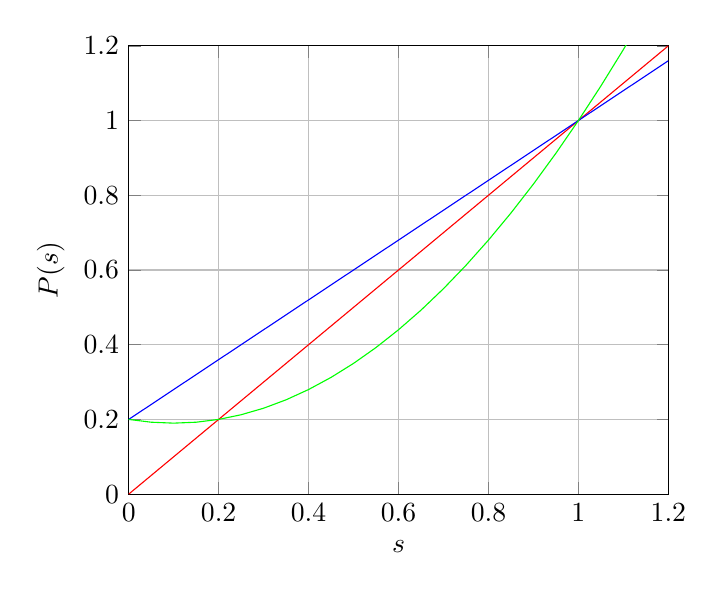
\begin{tikzpicture}[domain=0:1.2]
\begin{axis} [
    no markers, grid,
    xmax=1.2, ymax=1.2,
    xmin=0, ymin=0,
    xlabel={$s$},
    ylabel={$P(s)$}
    ]
\addplot +[red] plot (\x,\x);
\addplot +[blue] plot (\x,{0.2+0.8*\x});
\addplot +[green] plot (\x,{0.2 -0.2*x+ \x^2});
\end{axis}
\end{tikzpicture}
\caption{Cases for this problem where $p_0 =0.2$}
\end{figure}
The blue plot shows $m=P'(1) \leq 1$ and hence $q=1$.
The green plot shows $m = P'(1) >1$ and hence $q$ is the minimal non-negative solution for when there are multiple intersects.


Linking this to epidemic models, namely the SIR branching process.
Early in the spread of a novel infectious disease, virtually everyone in the population is susceptible. This motivates the linearisation of rates to produce an approximate CTMC.

Recall: infection at $\beta S I /(N-1) = \beta I(N-I-R)/(N-1)$\\
Recovery at $\gamma I$

We make the linearisation that the infection events occur at $\beta I$ in the early stages. We do not need to linearise recovery since it is already linear


So provided $N$ is sufficiently large, we have the approximate CTMC with\\
$I \to I+1$ at $\beta I$, and\\
$I \to I-1$ at $\gamma I$.
So now it is effectively a linear birth-death process. If we map this to a markovian branching process, we will consider a lifetime as the time until their next event, $\mu = \beta + \gamma$.
With probability of infection:
\[P_2 = \frac{\beta}{\beta + \gamma}\]
And probability of recovery
\[P_0 = \frac{\gamma}{\beta + \gamma} = 1- P_2\]


Hence 
\begin{align*}
    P(s) &= \sum_{k\geq 0} p_k s^k\\
        &=\frac{\gamma}{\mu} + \frac{\beta}{\mu} s^2\\
        P'(1) &= 2\beta/\mu = m
\end{align*}
\[M(t) = e^{\mu(2\frac{\beta}{\gamma} -1)t} = e^{(\beta-\gamma)t}\]
Which is effectively the same as what we got in early lectures, where $\beta-\gamma$ is the early growth rate of the epidemic.


Also
\begin{align*}
    \dd{F(s,t)}t &= \mu(P(F(s,t)) -F(s,t))\\
    \intertext{with } F(s,0)=s\\
    \dd{F(s,t)}t &= \gamma - (\beta + \gamma) F(s,t) + \beta F(s,t)^2 
    \intertext{Which is a Ricatti DE with solution}\\
    F(s,t)&=1 +\frac{(\gamma - \beta) (s-1)}{\beta(s-1)(\gamma - \beta s) e^{(\beta-\gamma)t}} 
\end{align*}

The probability of extinction, $q$ is the minimal non-negative solution to

\begin{align*}
    s = \frac{\gamma}{\mu} + \frac{\beta}{\mu} s^2\\
    \beta (s-1)(s-\frac{\gamma}{\beta}) = 0\\
    s = 1, \gamma/\beta\\
    \therefore q = \min\{ 1, \gamma/\beta\}
\end{align*}

How good is this approximation? What makes $N$ sufficiently large
\begin{itemize}
    \item During a minor outbreak, guaranteed for $\beta/\gamma \leq 1$, the epidemic `behaves' like the branching process for when $N$ is large,
    \item During a major outbreak, (requires $\beta/\gamma >1$) the epidemic grows like the branching process until about $\sqrt{N}$ members of the population become infected
\end{itemize}

\section{Household model}
2 Levels of `mixing' in the population.

In the normal (non household) model we have homogeneous mixing (everyone mixes equally with everyone else)

In the household (hh) model we have packages or groups of people who interact within the group with higher infection rates, and then smaller rates from outside of their group.

\begin{itemize}
    \item Population is split into groups
    \item 2 different rates of transmissions, typically within a hh the transmission rate is larger than between hhs\
    \item Let $M$ be the number of households. Assume that all the households are the same size (same number of people), $N$.
    \item So the total population is $MN$.
    \item We will assume $SIR$ dynamics.
\end{itemize}
How do we specify the state of the system?

The transition rates require knowing the hh epidemic structure for all hhs.

So what we need to know is the number of households of each possible configuration I.e. each possible $(S,i)$ combination. 
A single $hh$ can be in one of 
\[|S_h| = \frac{(N+1)(N+2)}2 = n\]
different configurations.


So the state of the HH process is specified as a vector $\vec m$ with elements $m_{(S,I)}$, corresponding to the number of hhs in each possible config.

And so $\vec m \cdot 1 = M$ where $M$ is the number of households.

\[\vec m = \left(m_{(N,0)},m_{(N-1,1)},\hdots, m_{(0,0)} \right)\]
So the length of $m$ should be the same size as the SIR model normally.
The state space is
\[S = \{\vec m \in \{0,\hdots,M\}^n : \sum_{j=0}^n m_j = M\}\]



\begin{table}[h]
    \centering
    \begin{tabular}{c|c|c}
         \emph{Event}&\emph{$\Delta$ state} & \emph{Rate}  \\
         \hline
         Within hh infection (of type $(S,I)$ & $ (m_{(S,I)}, m_{(S-1,I+1)}) \to (m_{(S,I)}+1, m_{(S-1,I+1)}+1) $ & $\frac{\beta SI}{(N-1)} m_{(S,I)} $\\
         \hline
         Between hh infection & $ (m_{(S,I)}, m_{(S-1,I+1)}) \to (m_{(S,I)}+1, m_{(S-1,I+1)}+1) $ & $\frac{\alpha S \ totalinf}{MN-1} m_{(S,I)}$\\
         \hline
         Recovery & $ (m_{(S,I)}, m_{(S,I-1)}) \to (m_{(S,I)}-1, m_{(S,I-1)}+1) $ & $\gamma I m_{(S,I)}$\\
    \end{tabular}
    \caption{Transitions for the household SIR model}
\end{table}
Where
\[totalinf = \sum_{(S,I)\in S_h} i m_{s,i}\]

You could change the $MN-1$ for the between hh infection rate based on different definitions for $\alpha,\beta$. But this would also change $totalinf$ and make it much grottier.

\subsection{Branching process approximation}
To make this approximation we require linear rates.

This works for everything except the between $hh$ infection rate.
Consider $M \to \infty$ and linearise
\begin{align*}
    q_B :&= \frac{\alpha S m_{(S,I)}}{MN-1} \sum_{(S,I)\in S_h} I m_{(S,I)}\\
    &\approx \frac{\alpha n m_{(N,0)}}{MN-1}  \sum_{(S,I)\in S_h} I m_{(S,I)}\\
    &\approx \frac{\alpha Mn }{MN-1}  \sum_{(S,I)\in S_h} I m_{(S,I)}\\
    &\approx \alpha  \sum_{(S,I)\in S_h} I m_{(S,I)}\\
\end{align*}
Households now also act independently of each other following the first infection (for the early stages).

We could analyse this as a multi-type Markovian branching process. Everything we have done will extend nicely to multi dimensional problems. But theres a simpler way as far as Josh is concerned.

We will look at this branching process approximation in a slightly different way. 



Recall for the SIR model an important parameter/measure/quantity is $R_0$. 

Where $R_0$ is the expected number of individuals infected by an infectious individual over their infectious period in an otherwise entirely susceptible population.

Recall $R_0$ is a threshold parameter, where
\begin{itemize}
    \item $R_0 >1$ implies a major outbreak is possible
    \item $R_0 \leq 1$ implies no major outbreak will occur 
\end{itemize}


Considering the hhs model, does $R_0$ act as a threshold parameter?
No it does not, 

New households are critical - try setting $\alpha = 0$ and $\beta > \gamma$. This will give $R_0 > 1$, without a major outbreak, since it is contained within a particular household.

We still want a threshold parameter so we will consider
$R_* =$ expected \# of hhs infected by a single hh that starts with 1 infectious individual and all others susceptible, over the hh epidemic. I.e. $I_h > 0$, assuming an otherwise entirely susceptible population.

Where $I_h$ is the number of infectious individuals in the first houseehold.

Under the assumptions of the household branching process, the rate at which new hhs are infected from the index household is
\[\alpha I_h(t)\]

Which is true since we have assumed there are infinitely many households


\[I_h(t) = I(X(t))\]
Where $X(t)$ is the within-hh CTMC epidemic process, and so $I(\cdot)$ is a function that maps the state space to the $\#$ of infectious individuals in that state.

Hence $\Omega$, the $\#$ of households infected by a single hh. I.e. $\mathbb{E}\left[\Omega\right] = R_*$, where $\Omega$ is a random variable which arises from an underlying inhomogeneous Poisson process with rate at time $t, \alpha I(X(t))$ which is also random.

So
\[\Omega \sim Poisson\left(\int_0^\infty \alpha I(X(t))dt\right)\]

Let 
\[D = \int_0^\infty \alpha I(X(t))dt\]

\begin{align*}
    R_* &= \mathbb{E}(\Omega)\\
    &= \mathbb{E}(D)\\
    &= \mathbb{E}\left[\alpha \int_0^\infty I(X(t))dt\right]
\end{align*}
With $X(0) = (N-1,1)$

Where $\int_0^\infty I(X(t))dt$ is a path integral of a CTMC.
So $R_*$ is the expected path integral of a CTMC.
We can calculate this easily apparently, but we need to derive shit first.


Another quantity of interest is the early growth rate, $r$ of the hh epidemic model. This is also known as the Malthusian parameter.

The Euler-Lotka equation is
\[b(t) = \int_0^\infty b(t-a) n(a) da\]
Where $b(t)$ is total expected number of external (between households) infections by time $t$, and $n(a)$ is the average (expected) rate at which external infections occur from an ``age'' $a$ hh. Where ``age'' means the time since first infection of the hh. 

The expected number of external infections grows at an exponential rate, $r$, so:

\begin{align*}
    b(t) &= b(t-a) e^{ra}\\
    \implies b(t) &= \int_0^\infty e^{-ra} b(t) n(a) da\\
    \implies 1 &= \int_0^\infty e^{-ra} n(a) da\\
    1 &= \mathbb{E} \int_0^\infty e^{-ra} \alpha I(X(a)) da
\end{align*}




HH Basic reproduction number, $R_*$ (under the branching process assumptions)
\[R_* = \mathbb{E} \left[\int_0^\infty \alpha I(X(t)) dt\right]\]
With $X(0) = (N-1,1)$
Where the inside of the expectation is a path integral (integrating over all possible paths).


Expectation of a path integral:

Let $X(t)$ be a CTMC with state space $S = A \cup B$ where $A$ consists of absorbing states, and $B$ is transient. (In the SIR $I=0$ is an absorbing state, and everything else is transient)

Assume we `earn' $f(k)$ per unit time that we spend in state $k\in S$, \\
with $f(k) = 0,\,\forall\, k\in A$.
Define
\[D = \int_0^\infty f(X(t)) dt\]
Where $D$ is the total amount `earned' over the life of the process. Note that $D$ is a random variable.



Example: considering a BD processs with state space $S = \{0,\ldots,N\}$ with $A = \{0\}$ and $B = \{1,\ldots,N\}$ hence $f(0) = 0$.
Let $f(k) = 1$ for all the other states.

What does $D$ represent? The expected time time until extinction.

\[D = \int_0^\infty 1_{\{X(t) >0\}} dt = \int_0^\tau 1 dt + \int_\tau^\infty 0 dt = \tau +0 =\tau\]
Where $\tau$ is the time the process becomes extinct in that realisation. Example finished.

Note that $D$ will always depend on the initial state $X(0)$.
Lets consider how to calculate the expected path integral conditioned on the initial state

\[d_i = \begin{cases}
        \mathbb{E}\left(D | X(0) = i\right), &i \in B\\
        0,&i \in A
    \end{cases}\]
Condition on the time of the next jump (first step analysis continuous analogue) at time $s$ and the state visited at that time, i.e. $j$.

\begin{align*}
\mathbb{E}\left(D | X(0) = i, X(u) = i, \forall\, 0<u<s, X(s) = j\right)&= f(i)s + \mathbb{E}(D|X(0)=j)\\
        &= f(i)s + d_j
\end{align*}
Now use LOTP to clean up the LHS - integrate out all $s$ and sum over all $j$. This gives
\begin{align*}
d_i &= \int_0^\infty\sum_{\substack{j\neq i\\j \in S}}\left[f(i)s + d_j\right]\frac{q_{ij}}{q_i}q_i e^{-q_i s} ds\\
&=\int_0^\infty\sum_{\substack{j\neq i\\j \in S}}f(i)s\frac{q_{ij}}{q_i}q_i e^{-q_i s} ds +\int_0^\infty\sum_{\substack{j\neq i\\j \in S}}d_j\frac{q_{ij}}{q_i}q_i e^{-q_i s} ds  \\
&=\int_0^\infty f(i)s q_i e^{-q_i s} ds +\sum_{\substack{j\neq i\\j \in S}}d_j\frac{q_{ij}}{q_i}\\
&=\frac{f(i)}{q_i} + \frac1{q_i} \sum_{\substack{j\neq i\\j \in S}} d_j q_{ij}\\
\implies d_iq_i &= f(i) +  \sum_{\substack{j\neq i\\j \in S}} d_j q_{ij}\\
\implies d_iq_i &= f(i) +  \sum_{\substack{j\neq i\\j \in B}} d_j q_{ij}\\
Q_B \mathbf{d} = - \mathbf{f}\\
\mathbf{d} = -\mathbf{f} \backslash Q_B
\end{align*}
Where $Q_B$ is $Q$ restricted to the states in $B$ (i.e. remove all rows and columns relating to $A$). $\mathbf{d} = (d_i,i\in B)$ and $\mathbf{f} = (f(i),i\in B)$


The expected total amount `earned' over the life of the process, conditioned on starting in state $i$ satisfies a system of linear equations.  


Exercise: Let $S = \{0,1,2,3\}$ in a BD process
\[q_{i,j} = \begin{cases}
a,& j=i+1, i=1,2\\
b,& j=i-1, i=1,2,3\\
\end{cases}\]
Evaluate the expected time to extinction.
This will be $d_0$ for $f(i) = 1$ for $i\neq 0$ and $f(0) = 0$.

\[Q = \begin{pmatrix}
    0&0&0&0\\
    b & -(a+b) & a & 0\\
    0&b & -(a+b) & a\\
    0&0&b & -(a+b)\\
\end{pmatrix}\]
Hence
\[Q_B = \begin{pmatrix}
    -(a+b) & a & 0\\
    b & -(a+b) & a\\
    0&b & -b\\
\end{pmatrix}\]


So
\begin{align*}
    Q_B \mathbf{d} = -\mathbf{1}\\
    (-a+b) d_1 + ad_2 = -1\\
    b d_1 - (a+b) d_2 + ad_3 = -1\\
    bd_2 - bd_3 = -1
\end{align*}

Which I cbf solving but good enough

Now assume there is some cost related to the number of individuals in the population. This just changes $\mathbf{f}$, and nothing else.


Distribution of the Path integral


Lets consider the distribution of $D$. Use the Laplace-Stieltjes transform (LST) of $D$:
\[L = \mathbb{E}\left(e^{-lD}\right)\] 
Where $l$ is a complex variable and is the parameter of the transform?

\[\text{let  } L_i = \mathbb{E}\left(e^{-lD} | X(0) = i\right)\]
Note that $L_i = 1$ for all $i \in A$ (remember $D_i = 0$ so $e^{0} = 1$)


As before, we have
\begin{align*}
&\mathbb{E}\left(e^{-lD} | X(0) = i, X(u) = i , \, 0<u<s, \, X(s) = j\right)    \\
&= \mathbb{E}\left(e^{-l(f(i)s + D)} | X(0) = j\right)\\
&= e^{-lf(i)s}\mathbb{E}\left(e^{-lD} | X(0) = j\right)\\
&= e^{-lf(i)s} L_j
\end{align*}
Now use LOTP to clean up the first line
\begin{align*}
    L_i &= \int_0^\infty \sum_{j\neq i} \left[e^{-lf(i)s} L_j\right] \frac{q_{ij}}{q_i} q_i e^{-q_is} ds\\
    &=\int_0^\infty  e^{-s(lf(i)+q_i)} ds\sum_{j\neq i}L_j q_{ij} \\
    &= \frac{1}{l f(i)+ q_i} \sum_{j\neq i} q_{ij} L_j\\
    (l f(i) + q_i) L_i &= \sum_{j\neq i} q_{ij} L_j\\
    (Q_b - lF)\mathbf{L} &= - \mathbf{a}
\end{align*}

Where $Q_B$ is as before, $l$ is the LST parameter, $F$ is:
\[F = \begin{pmatrix}
    \ddots & \\
    &\ddots&&0\\
    &&\vec{f_b}&&\\
    &0&&\ddots\\
    &&&&\ddots 
\end{pmatrix}\]

And $\vec{a}$ is:
\[\vec a = \left(- \sum_{\substack{j\neq 1\\ j\in A}} q_{ij}, \quad i\in B\right)\]

Exercise:
$S = \{0,1,2,3\}$
\begin{align*}
    q_{i,i+1} = a,\quad i=1,2\\
    q_{i,i-1} = b,\quad i=1,2,3
\end{align*}
Write down the system of linear equations for the LST of the time to extinction. (given 0 is an absorbing state)
\[Q = \begin{pmatrix}
    0&0&0&0\\
    b & -(a+b) & a & 0\\
    0&b & -(a+b) & a\\
    0&0&b & -(a+b)\\
\end{pmatrix}\]
Hence
\[Q_B = \begin{pmatrix}
    -(a+b) & a & 0\\
    b & -(a+b) & a\\
    0&b & -b\\
\end{pmatrix}\]

\[F=diag(1,1,1,1)\]
\[L = \begin{pmatrix}
    L_1\\L_2\\L_3
\end{pmatrix}\]
\[a = - \begin{pmatrix}
    b\\0\\0
\end{pmatrix}\]


And ceebs expanding that bs




To evaluate the distribution, we need to invert the LST.

We will consider a particular metod. But new methods exist which might be better




Let
\[\hat{f}_D (l) = \mathbb{E}\left(e^{-lD}\right) = \int_0^\infty e^{-ld} f_D(d) dd\]
Where $l = \gamma + iu$

The inverse of the Laplace tranform (i.e. the integral) is given by the Bromwich inversion integral.
\[f_D(x) = \frac{1}{2\pi i} \int_{\gamma - i\infty}^{\gamma +i\infty} e^{lx} \hat{f}_D (l) dl\]
Where $\gamma$ is greater than the real part of all singularities of $\hat{f}_D(l)$

Effectively, we now use a trapezoidal rule.
Substitute $l = \gamma + iu$ so $dl = idu$
\begin{align*}
f_D(x) &= \frac{1}{2\pi} \int_{-\infty}^\infty e^{(\gamma + iu)x} \hat{f}_D(\gamma+iu) du\\
&= \frac{e^{\gamma x}}{2\pi} \int_{-\infty}^\infty (\cos(ux) + i\sin(ux)) \hat{f}_D(\gamma + iu) du\\
\text{(Real and nonnegative)}&\\
&=\frac{2e^{\gamma x}}{2\pi} \int_0^\infty R(\hat{f}(\gamma+iu)) \cos(ux) du\\
\text{(Apply the trapezoidal rule w step size )}&h = \pi/2x, \, \gamma = a/2x\\
f_D(x) &\approx \frac{e^{a/2}}{2x} R(\hat{f}(a/2x)) + \frac{e^{a/2}}{x} \sum_{k=1}^\infty (-1)^k R(\hat{f}\left((a+2k\pi i)/2x)\right)
\end{align*}
Which we would do with matlab.


Exercise: A single individual (SIR).
Assume they are infectious for an exponentially distributed time with mean $1/\gamma$. And during their infectious period, they infect new individuals at rate $\beta$.
Let $X(t)$ be 1 if infectious, 0 if recovered. $S = \{0,1\}$ 
\begin{enumerate}
    \item What is the expected number of secondary infections directly from the first individual?
    $q_{1,0} = \gamma$ , $X(0) =1$

    $f(1) = \beta$, $f(0) = 0$
    \[R_0 = \mathbb{E}\left[\int_0^\infty \beta X(t) dt\right] = \mathbb{E}\left[\int_0^\infty f(X(t)) dt\right]\]
    So this is a single linear equation to solve

    \item What is the pmf of the number of secondary infections directly from the first individual?
    $N_s \sim Poi(D)$ where 
    $N_s$ is the number of secondary infections, and 
    \[D = \int_0^\infty f(X(t)) dt\]

\end{enumerate}



Recall
\[D = \int_0^\infty f(X(t)) dt\]
Where $X(t)$ is a CTMC with $S = A\cup T$, where $A$ consists of absorbing states, and $T$ consists of transient states, and the function $f(k)$ is the amount `earned' per unit time while in state $k\in S$. $f(k) = 0 \ \forall \ k \in A$

We derived:
\[Q_T \mathbf{d} = - \mathbf{f}\]
Where $Q_T$ is the $Q$ matrix restricted to transient states (removing the rows and columns associated with $A$). 

$\mathbf{d} = (d_i, i \in T)$, such that $d_i = \mathbb{E}(D | X(0) = i)$. So
\[R_* = \mathbb{E}\left[\int_0^\infty \alpha I(X(t)) dt\right]\]
Can evaulate $R_*$ by solving a system of linear equations.

For $N=1$ we got $R_* = \frac{\alpha}{\gamma} = R_0$

(Since $N=1$ is basically just the SIR model)


Now, we have
\[ \mathbb{E}\left[\int_0^\infty e^{-rt} \alpha I(X(t)) dt\right]=1\]
The LHS is equivalent to the path integral of the original process, but modified so that from each state $i\in T$, we have a rate $r$ of entering some arbitrary state in $A$.


As an example, $N=1$:

Recall the early growth rate $r = \beta- \gamma$. I.e. $I(t) = I(0) e^{rt}$ early on.

Recall $X(t)$ is an indicator of infections. $S = \{0,1\}$ and $q_{1,0} = \gamma$

So 
\[D = \int_0^\infty \beta X(t) dt\]

I.e. $f(1) = \beta$ and $f(0) = 0$

\[Q = \begin{pmatrix}
    0&0\\ \gamma & -\gamma
\end{pmatrix}\]
\[Q_T \mathbf{d} = - \mathbf{f}\]
\[-\gamma R_0 = -\beta\]
And hence
\[R_0 = \beta/\gamma\]

For the modified process (for the LHS of that equation), it changes to $q_{1,0} = \gamma + r$ since we enter the system at rate $r$.
\[Q^* = \begin{pmatrix}
    0&0\\r + \gamma & - r- \gamma
\end{pmatrix}\]

Since we have incorporated this rate, the integral becomes 
\[d=\mathbb{E}\left[\int_0^\infty \alpha I(X^*(t)) dt\right]=1\]
\[-(\gamma + r)d = -\alpha\]
\[d = \frac{\alpha}{\gamma+r} = 1 \implies r = \alpha- \gamma\]


A different way to calculate the offspring distribution

Recall, $N_s \sim Poi(D)$ (where $N_s$ is the number of secondary infections). So:

\[P(N_s = k) = \int_0^\infty\frac{e^{-x}x^k}{k!} f_D(x) dx\]
We used the LST (laplaces stieljes transform) of $D$
\[\mathbb{E}(e^{-lD} | X(0) = i)\]
And we showed there was a system of linear equations which this would satisfy.
Then we could invert the LST (using the Euler method) to give us $f_D(x)$.
Then we would have to integrate this numerically.

This is extremely computationally demanding.



Note that 
\begin{align*}
  P(N_s =k) = \frac1{k!} \mathbb{E}\left[D^k e^{-D}\right]
\end{align*}
And that 
\[L = \mathbb{E}\left[e^{-lD}\right]\]

Hence,
\[\frac{dL}{dl} = \mathbb{E}\left[-De^{-lD}\right]\]
giving
\[-1 \times \frac{dL}{dl} \pipe_{l=1} = P(N_s=1)\]
Similarly,

\begin{align*}
    \frac{d^2L}{dl^2} = \mathbb{E}\left[D^2 e^{-lD}\right]\\
    (-1)^2\frac12 \frac{d^2 L }{dl^2} = P(N_s=2)\\
    \vdots\\
    (-1)^k \frac{1}{k!} \frac{d^kL}{dl^k} = P(N_s=k)    
\end{align*}


Recall
\[l f(i) L_i = \sum_{j\in T} q_{ij} L_j + \sum_{j\in A} q_{ij}, \quad i\in T\]
Differentiating with respect to $l$ gives
\[f(i) L_i + l f(i) \frac{dL_i}{dt} = \sum_{j\in T} q_{ij} \frac{dL_i}{dt}\]

Going to use $L_i^{(n)} : = \frac{d^n L_i}{dl^n}$ as shorthand

\[f(i) L_i^{(1)} + \sum_{j\in T} q_{ij} L_j^{(1)} - f(i) L_i\]

Differentiating again gives
\[f(9i) L_i^{(2)} + l f(i) L_i^{(2)} = \sum_{j\in T} q_{ij} L_j^{(2)} - f(i)L_i^{(1)}\]
\[\implies lf(i) L_i^{(2)} = \sum_{j\in T} q_{ij} L_j^{(2)} - 2f(i) L_i^{(1)}\]
And in general
\[l f(i) L_i^{(m)} = \sum_{j\in T} q_{ij} L_j^{(m)} - m f(i) L_i^{(m-1)}, \quad i \in T, m \geq 1\]


Exercise ($N=1$)

Recall
\[L_1 = \frac{\gamma}{\gamma + l \beta}\]
Use the recursive method to verity:
\[P(N_s = k) = \frac{\gamma \beta^k}{(\beta+\gamma)^{k+1}}, \quad k=0,1,\hdots\]


Hence, in place of numerical integration of numerical Laplace inversion of a solution of a system of linear equations. We can recursively solve systems of linear equations.


\subsection{Final Size Distribution}
The distribution of the total number of people who get infected over the course of an outbreak.

For the SIR model:
We assume transitions at $\beta SI$ and $\gamma I$ for infection and recovery respectively.

If we consider $DA$ mapping, this will effectively be the probability of ending on each diagonal state.
I.e. those where $Z_1 = Z_2$.

We don't need to consider duration or any time factors, just the jump chain behaviour.

Consider the jump chain, $A$
\[A = \left(a_{ij}, i,j \in S\right) \ st \ a_{ij} = \frac{q_{ij}}{q_{i}} \ \& \ a_{ii} = 0\]

Let $p_i$ be the probability of ever reaching (or hitting) state $I$. Then
\[p_i = b_i + \sum_{j\neq i} p_j a_{ji}\]
Where $b_i$ is the probability of starting in state $i$.
\[\vec p (I-A) = \vec b \]
The matrix $A$ is strictly upper triangular, so this system can be solved via forward substitution.

The final size distribution involves taking the entries from $\vec p$ corresponding to absorbing states (where $Z_1=Z_2$)
Here
\[P(F=j) = P_{j(2N+3-j)/2 +1}\]
for $j=0,\hdots,N$

Rather than storing $A$, we can use the structure of the state space to update, as:
 Set $\vec p = \vec b$
\begin{align*}
    p_{i+1} = p_{i+1} + p_ia_{i,i+1}\\
    p_{i+N - Z_2(i)} = p_{i+N-Z_2(i)} + p_i(1-a_{i,i+1})    
\end{align*}
For $i=2,\hdots,(N+1)(N+2)/2$. This is different to forward substitution. By doing this we don't have to store the matrix $A$.

We can reduce the storage even further:
Each step in the iterative scheme calculates the probabilities of transitions to `connected' states when we are in state $i$.
Once we have iterated through state $i$, we can free the memory from $p_i$ and its jump probabilities, unless $i$ is absorbing.
We only need a vector of length $N+1$ (the length of the final size distribution) for the whole problem.

E.g. if we have $q_2 =1$ (i.e. we start with 1 infectious and $N-1$ susceptible).
Set $q_2 = 1$, $q_i = 0$ otherwise.
First step:
\begin{align*}
    q_3 = q_3 + q_2 a_{23}
    q_2 = q_2a_{25} = q_2(1-a_{23}) 
\end{align*}
Where $q_2$ now holds the probability of being absorbed in in state $5$.

So in full colexicographical numbering: 
\begin{verbatim}
    for Z2 = 0:N
        for Z1 = Z2+1 : N-1
            q(Z1+2) = q(Z1+2) + q(Z1+1)*a(Z1+1,Z1+2)
            q(Z1+1) = q(Z1+1)*(1-a(Z1+1,Z1+2))
        end
    end
    a(Z1+1,Z1+2) = @(Z1,Z2) 
\end{verbatim}
\begin{align*}
    (z_1,z_2) \to (z_1+1, z_2) &= \frac{\beta(N-z_1)(z_1-z_2)}{\beta(N-z_1)(z_1-z_2) + \gamma(z_1-z_2)}\\
    &=\frac{\beta(N-z_1)}{\beta(N-z_1) + \gamma}\\
    &=\frac{1}{1 + \frac{\gamma}{\beta(N-z_1)}}\\
    &=\frac{1}{1 + \frac{1}{R_0(N-1) (N-z_1)}}\\
\end{align*}


\section{Inference}
We may be able to specify the model for the dynamics of a system, but to provide insights to a particular system, we need to know something about the parameter values for the system.


We may have some observations/data from the system which we wish to use to infer the parameters (or alternatively their distribution). In deterministics we may refer to this as an `inverse problem'.

We will focus specifically on Bayesian inference (which Josh believes is the best kind), but today we will start with Frequentist (classical) inference. 

From a text:

\begin{verse}
\noindent
{\centering
In Classical inference, model parameters are regarded as fixed quantities. The values of the parameters are estimated from data using estimators that are random variables, \& whose distributional properties \textit{may} be known}\\
- O'Neill (2002)
\end{verse}
The main approach to inference in this setting is Maximum likelihood estimation. 

The likelihood (of parameters $\theta$) is the probability of observing the data, $D$, given a specified model with parameters $\theta$.

The likelihood function, $L(\theta) = P(D|\theta)$.

If the data $D = (d_j,j=1,\ldots,n)$ correspond to independent random variables, $X_1,\ldots,X_n$, then
\[L(\theta) = \prod_{i=1}^n P(X_i(\theta) = d_i)\]

For example lets assume independent outbreaks of the same disease in $n$ populations which are identical with respect to epidemiologically important characteristics, except for the population sizes.

We observe the final size in each population, know the respective population sizes, and assume SIR dynamics:

\[L(R_0) = \prod_{i=1}^n P(F_{n_i}(R_0)) = d_i\]
The `best' estimate of $R_0$ from this data is the one that maximises $L(R_0)$, referred to as the MLE (maximum likelihood estimate)

We often work with the log likelihood
\[\ell(R_0) = \log(L(R_0)) \stackrel{indep}= \sum_{i=1}^n \log \left(P(F_{n_i}(R_0)) = d_i\right)\]
And we still want to maximise this function.


Confidence intervals can be constructed, say using profile-likelihood based CIs, or more commonly they are approximated by asymptotic normality and inverse of the Fisher information (matrix) is the var/cov matrix.


Example:

Assume we flip a coin (iid) $N=30$ times, and we observe $s=7$ heads. What is the MLE for the binomial probability (of getting a head)?
We can say it will be
\[\hat{p} = \frac s N = \frac7{30}\]
\begin{align*}
    L(p) = \ncr Ns p^s (1-p)^{N-S}\\    
\end{align*}
We want to maximise this function. Take the derivative and set to $0$. Should get the same value.


SIR outbreak. Estimate (using MLE) of $R_0$ given the following final size and population size pairs:
\begin{align*}
    (6,10), (20,&20), (47,50),\\
    (1,30), (38,40), & (90,100), (5,16)\\
\end{align*}




What is the likelihood function of a CTMC, where we observe the state of the system of the process at a sequence of times, $t_1,\ldots,t_n$











































\end{document}
